% THIS DOCUMENT IS FOLLOWS THE VOLERE TEMPLATE BY Suzanne Robertson and James Robertson
% ONLY THE SECTION HEADINGS ARE PROVIDED
%
% Initial draft from https://github.com/Dieblich/volere
%
% Risks are removed because they are covered by the Hazard Analysis
\documentclass[12pt]{article}
\usepackage[parfill]{parskip}

%\usepackage[pdftex]{graphicx}
%\graphicspath{{../pdf/}{D:\ImagesforProjectLatex}}
 %\DeclareGraphicsExtensions{.pdf,.jpeg,.png}
\usepackage{graphicx}
\usepackage{makecell}

\usepackage{booktabs}
\usepackage{tabularx}
\usepackage{hyperref}
\hypersetup{
    bookmarks=true,         % show bookmarks bar?
      colorlinks=true,      % false: boxed links; true: colored links
    linkcolor=red,          % color of internal links (change box color with linkbordercolor)
    citecolor=green,        % color of links to bibliography
    filecolor=magenta,      % color of file links
    urlcolor=cyan           % color of external links
}

\newcommand{\lips}{\textit{Insert your content here.}}

%% Comments

\usepackage{color}

\newif\ifcomments\commentstrue %displays comments
%\newif\ifcomments\commentsfalse %so that comments do not display

\ifcomments
\newcommand{\authornote}[3]{\textcolor{#1}{[#3 ---#2]}}
\newcommand{\todo}[1]{\textcolor{red}{[TODO: #1]}}
\else
\newcommand{\authornote}[3]{}
\newcommand{\todo}[1]{}
\fi

\newcommand{\wss}[1]{\authornote{blue}{SS}{#1}} 
\newcommand{\plt}[1]{\authornote{magenta}{TPLT}{#1}} %For explanation of the template
\newcommand{\an}[1]{\authornote{cyan}{Author}{#1}}

%% Common Parts

\newcommand{\progname}{ProgName} % PUT YOUR PROGRAM NAME HERE
\newcommand{\authname}{Team \#, Team Name
\\ Student 1 name
\\ Student 2 name
\\ Student 3 name
\\ Student 4 name} % AUTHOR NAMES                  

\usepackage{hyperref}
    \hypersetup{colorlinks=true, linkcolor=blue, citecolor=blue, filecolor=blue,
                urlcolor=blue, unicode=false}
    \urlstyle{same}
                                


\begin{document}

\title{Software Requirements Specification for \progname: subtitle describing software} 
\author{\authname}
\date{\today}
	
\maketitle

~\newpage

\pagenumbering{roman}

\tableofcontents

~\newpage

\section*{Revision History}

\begin{tabularx}{\textwidth}{p{3cm}p{2cm}X}
\toprule {\textbf{Date}} & {\textbf{Version}} & {\textbf{Notes}}\\
\midrule
Oct 11, 2024 & 1.0 & Initial Creation - Final\\
\bottomrule
\end{tabularx}

~\\

~\newpage
\section{Purpose of the Project}
\subsection{User Business}
The primary business of the McMaster GSA softball league is to facilitate recreational softball activities for students, staff, and alumni. The league aims to provide an organized platform for scheduling games, managing teams, and tracking player performance, enhancing the overall experience for participants. By streamlining league operations, the platform will foster a more inclusive and efficient environment, enabling better communication among players, captains, and commissioners.\
\begin{itemize}
  \item Team Management: captains will have the ability to create and manage their teams, inviting players to join, assigning roles, and ensuring that all team members are informed about practices and games.
  \item Game Scheduling: users will utilize the scheduling tools to view upcoming games, propose new times, and request rescheduling, ensuring that all participants are aware of their commitments and can manage their time effectively.
  \item Communication and Announcements: Commissioners will post league-wide announcements and updates, allowing all users to stay informed about important news, such as changes in scheduling, league policies, or events.
  \item Performance Tracking: players can track their individual and team performance through leaderboards and standings, fostering a sense of competition and motivation to improve.
  \item Payment Management: the application will provide visibility into players' payment statuses, enabling captains and commissioners to easily monitor team compliance with league participation requirements.
  \item Community Building: through features such as announcements and event notifications, users can engage with one another beyond the field, strengthening community ties and enhancing the overall experience of league participation.
\end{itemize}
\subsection{Goals of the Project}
The primary goal of the McMaster GSA softball league platform project is to develop an intuitive, user-friendly web application that enhances the management and operation of the league. Specific goals include:
\begin{itemize}
  \item Streamlined Scheduling and Communication: Simplify the scheduling process for games and practices, allowing captains to manage their teams effectively while facilitating clear communication between all stakeholders.
  \item Role-Based Access Control (RBAC): Implement a secure login system using JSON Web Tokens (JWT) that allows different levels of access for commissioners, captains, and players, ensuring that users can perform actions relevant to their roles without compromising sensitive information.
  \item Improved User Interface: Design a modern, responsive user interface that enhances usability and engagement, making it easier for participants to navigate the platform and access essential features.
  \item Enhanced Data Management: Develop robust features for managing player registrations, tracking payment statuses, and maintaining accurate standings and leaderboards, thereby reducing administrative overhead and increasing transparency.
  \item Facilitate Community Engagement: Foster a sense of community among participants through features such as announcements, event notifications, and an organized platform for sharing updates, enhancing the overall experience of league participation.
\end{itemize}

\pagebreak

\section{Stakeholders}
\subsection{Client}
The client for this project is the McMaster GSA, which oversees the softball league. Their primary goal is to provide a robust platform that improves the management of the league, facilitates better communication among users, and enhances the overall user experience. The GSA will benefit from increased participation and smoother operations, ultimately fostering a stronger community at McMaster.
\subsection{Customer}
The customers are the users of the platform, including players, captains, and commissioners. They seek an intuitive and efficient system that allows for easy management of games, team coordination, and communication. By addressing their needs, the platform aims to increase user satisfaction and engagement within the league.
\subsection{Other Stakeholders}
Other stakeholders include the university administration, potential sponsors, and the broader McMaster University community. These groups may have a vested interest in the successful operation of the league, as it contributes to student life and community engagement. Sponsors may seek visibility and promotional opportunities through the league's activities.
\subsection{Hands-On Users of the Project}
Hands-on users include the players, captains, and commissioners who will interact with the platform daily. Players will use the system to join teams, view schedules, and track their performance. Captains will manage their teams, schedule games, and communicate with players. Commissioners will oversee league operations, post announcements, and manage administrative tasks.
\subsection{Personas}
Player Persona: A student looking to join a team, participate in recreational activities/games, check their game schedule, and track their performance.
Captain Persona: An organized individual responsible for managing team logistics, rescheduling games, and ensuring effective communication.
Commissioner Persona: A knowledgeable overseer who ensures the league operates smoothly, creates game schedules, handles disputes, and communicates important updates to all users.
\subsection{Priorities Assigned to Users}
Players prioritize ease of joining teams, checking their game schedule, and tracking performance.
Captains focus on scheduling flexibility, team management features, and communication tools.
Commissioners prioritize administrative functionality, announcement features, and overall system reliability.
\subsection{User Participation}
User participation will be critical throughout the project. Stakeholders will provide feedback during the development process to ensure the platform meets their needs. User testing sessions will be conducted to gather insights and refine the interface and features.
\subsection{Maintenance Users and Service Technicians}
Maintenance users include any staff responsible for ongoing system updates, bug fixes, and technical support (our team). This group ensures that the platform remains functional, secure, and up-to-date. Service technicians may be involved in troubleshooting issues and providing assistance to users, particularly during peak usage periods, such as the beginning of the season.

\section{Mandated Constraints}

\subsection{Solution Constraints}
Constraints that limit the design of the solution:
\begin{itemize}
    \item \textbf{Scalability}: The initial version of the platform must support 30-40 teams, with future scalability to accommodate more teams.
    \item \textbf{Device Accessibility}: The system must be optimized for desktops, tablets, and mobile phones.
\end{itemize}

\subsection{Implementation Environment of the Current System}
The current implementation environment includes:
\begin{itemize}
    \item \textbf{Operating Systems}: Compatibility with Windows, macOS, Android, and iOS.
    \item \textbf{Supported Browsers}: The platform must be fully functional on Chrome, Firefox, Safari, and Edge.
    \item \textbf{Hosting Environment}: The platform will continue to use the existing hosting environment, which has already been established for the current website. No changes to the hosting infrastructure are anticipated unless new features require additional support.
\end{itemize}

\subsection{Partner or Collaborative Applications}
There are no partner or collaborative applications required for this project.

\subsection{Off-the-Shelf Software}
No off-the-shelf software will be utilized for payment handling or calendar integration.

\subsection{Anticipated Workplace Environment}
The platform is anticipated to be used in various environments:
\begin{itemize}
    \item \textbf{Users}: The platform will be accessed by league commissioners, team captains, players, and administrators.
    \item \textbf{Device Types}: Users are expected to use the platform on personal laptops, desktops, and mobile devices.
\end{itemize}

\subsection{Schedule Constraints}
The project is constrained by a strict timeline, with key milestones that must be met:
\begin{itemize}
    \item \textbf{Development Timeline}: The platform must be completed within the designated course timeline (approximately 8 months).
    \item \textbf{Fixed Milestones}: Deliverables must be submitted according to predefined deadlines.
\end{itemize}

\subsection{Budget Constraints}
There are no budget constraints applicable to this project. The existing infrastructure and hosting environment will be reused, and no additional licensing fees are required.

\subsection{Enterprise Constraints}
\begin{itemize}
    \item \textbf{Hosting Environment}: The platform must utilize the existing hosting environment already set up for the current system, which may come with certain limitations or capabilities that need to be respected.
    \item \textbf{No External Sponsorship}: There is no specific enterprise funding or sponsoring this project, meaning there are no additional budgetary or compliance constraints from an external organization.
\end{itemize}

\section{Naming Conventions and Terminology}

\subsection{Glossary of All Terms, Including Acronyms, Used by Stakeholders involved in the Project}
The following terms are used consistently throughout this document:
\begin{itemize}
    \item \textbf{Commissioner}: Manages the entire league and oversees operations.
    \item \textbf{Captain}: Responsible for team management, including schedules and rosters.
    \item \textbf{Player}: A participant in a team who needs access to schedules and standings.
    \item \textbf{Schedule Slot}: The specific time allocated for a game.
    \item \textbf{Waiver}: A document that participants must sign before joining the league.
\end{itemize}

\section{Relevant Facts and Assumptions}

\subsection{Relevant Facts}
\begin{itemize}
    \item \textbf{Role Definition}: Specific roles such as commissioner, captain, and player exist within the system, each with unique permissions and responsibilities.
    \item \textbf{Season Timeline}: The platform will primarily be used during the softball season from April to September.
\end{itemize}

\subsection{Business Rules}
\begin{itemize}
    \item \textbf{Team Registration}: Teams must be registered by captains before the league starts.
    \item \textbf{Scheduling Requests}: Rescheduling requests must be made at least 48 hours in advance.
\end{itemize}

\subsection{Assumptions}
\begin{itemize}
    \item \textbf{Internet Access}: All users are assumed to have access to a stable internet connection.
    \item \textbf{Mobile Usage}: It is assumed that many users will access the platform using mobile devices, so a mobile-friendly interface is required.
    \item \textbf{Payment Compliance}: Players are expected to make payments via e-transfer, which will be managed externally. The platform will include an interface for the designated staff member to track which players have completed their payments, without integrating any direct payment gateway. Manually updated payment status is assumed to be correct.
\end{itemize}

\section{The Scope of the Work}
\subsection{The Current Situation}
The current implementation of the GSA softball league platform is run on outdated software.
This issue makes the management of the league platform difficult without a certain degree of
programming knowledge. The purpose of the GSA softball platform is to manage the softball
league functionalities (communication, scheduling, player logins, etc.) so it meets the needs
and demands of the league.
\subsection{The Context of the Work}
See \textit{Figure 1.}
\begin{figure}
	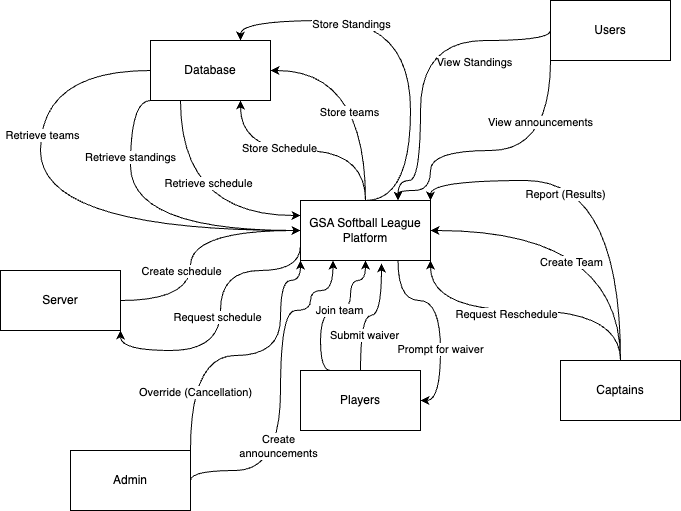
\includegraphics[width=\linewidth]{Context_diagram.png}
	\caption{Context diagram.}
	\label{fig:context_diagram}
\end{figure}
\pagebreak
\subsection{Work Partitioning}
\begin{center}
    \begin{tabular}{ |c|c|c| }
        \hline
        \textbf{Event Name}  & \textbf{Input/Output} & \textbf{Summary} \\
        \hline
        Login & \makecell{User ID (IN) \\ Password (IN)}
		& \makecell{Enter user ID and password.
		\\User is created and user data
		\\is stored in the database.} \\
        \hline
		Join team & \makecell{User Login (IN) \\ Prompt for waiver (OUT) \\ Submit waiver (IN)}
		& \makecell{User logs in as a player, then
		\\completing the waiver allows
		\\the user to join a team} \\
		\hline
        Create team & \makecell{User Login (IN) \\ Team Info (IN)}
		& \makecell{User logins into the system as
		\\a captain, then the user inputs
		\\the team info to create a team.
		\\The team is created and stored
		\\in the database.} \\
		\hline
        Create Schedule & Season Schedule (OUT)
		& \makecell{System uses all teams info to
		\\create season-long schedule
		\\with all open slots available.} \\
		\hline
        Override & Admin credentials (IN)
		& \makecell{User inputs admin credentials
		\\and gets access to complete
		\\override.} \\
		\hline
        Create announcement & \makecell{Admin credentials (IN)
		\\Announcement details (IN) \\Publish announcement (OUT)}
		& \makecell{User inputs admin credentials
		\\to gain access then enters
		\\in the announcements details.
		\\Then the announcement is
		\\published on the web page.} \\
		\hline
        Request reschedule & User Login (IN) 
		& \makecell{User logs into the system as
		\\a captain, then creates a
		\\request to reschedule a game
		\\in an open slot.}\\
		\hline
        Report (Results) & \makecell{User Login (IN)
		\\ Game results (IN) \\ Update standings (OUT)}
		& \makecell{User logs in as a captain then
		\\inputs the results of the game.
		\\Update standings in the database
		\\with reported results.} \\
        \hline
    \end{tabular}
\end{center}

\subsection{Specifying a Business Use Case}
The primary business use case for this platform is to efficiently manage all aspects of league operations from player registrations to game scheduling in a user-friendly and streamlined manner. The platform will provide commissioners, team captains, and players with a centralized system to interact with the league. The system allows commissioners to oversee the entire league, manage team and player information, and handle payments. Team captains will be able to manage their rosters, submit rescheduling requests, and report game scores, while players can join teams, view schedules, and observe league rankings and scores.
For example, team captains can log in to the platform and create their teams. Players can join a team by requesting approval from the captain, while commissioners can monitor the overall progress and approve team formations. Throughout the season, captains can report game scores directly into the system, which automatically updates the standings. If a team needs to reschedule a game, the captain can request a change through the system, selecting from available timeslots. The system will queue the request for commissioner approval and update the schedule once the rescheduling is confirmed.

\section{Business Data Model and Data Dictionary}
\subsection{Business Data Model}
\begin{itemize}
    \item \textbf{User}
    \begin{itemize}
        \item UserID: Unique identifier for each user.
        \item Name: Full name of the user.
        \item Email: Email address used for communication and login.
        \item Role: The role of the user in the system (commissioner, captain, player).
        \item TeamID: The ID of the team the user is affiliated with (for captains and players).
    \end{itemize}
    
    \item \textbf{Team}
    \begin{itemize}
        \item TeamID: Unique identifier for each team.
        \item TeamName: Name of the team.
        \item Division: The division the team is assigned to.
        \item CaptainID: The UserID of the team captain.
        \item Roster: List of players (UserIDs) on the team.
    \end{itemize}
    
    \item \textbf{Game}
    \begin{itemize}
        \item GameID: Unique identifier for each game.
        \item TeamAID: The ID of the first participating team.
        \item TeamBID: The ID of the second participating team.
        \item Date: The date the game is scheduled.
        \item Time: The time the game is scheduled.
        \item Result: The outcome of the game (win/loss/tie) reported by captains.
        \item ScoreTeamA: The score of Team A in the game.
        \item ScoreTeamB: The score of Team B in the game.
    \end{itemize}
    
    \item \textbf{Schedule}
    \begin{itemize}
        \item ScheduleID: Unique identifier for the schedule.
        \item GameID: The ID of the game scheduled.
        \item SlotNumber: The slot number for the game (time and location).
        \item AvailableSlots: List of available time slots for potential rescheduling.
    \end{itemize}
    
    \item \textbf{Standing}
    \begin{itemize}
        \item TeamID: The ID of the team.
        \item Wins: Number of games won by the team.
        \item Losses: Number of games lost by the team.
        \item Ties: Number of tied games.
        \item Rank: Current rank of the team in the league.
        \item TotalScore: Cumulative score across all games, used to break ties in standings.
    \end{itemize}
\end{itemize}

\subsection{Data Dictionary}
\begin{itemize}
    \item \textbf{Users:} There are three types of users: commissioners, team captains, and players. Commissioners oversee league operations, team captains manage their respective teams, and players join and participate in games. Each user has attributes such as name, email, role, and team affiliation.
    
    \item \textbf{Teams:} Teams consist of players and a captain. Teams are scheduled to play games, and the results of those games contribute to league standings. Teams have attributes like team name, captain, and roster.
    
    \item \textbf{Games:} Games represent the scheduled matches between two teams. Each game has attributes like date, time, and the teams involved, as well as the final score for both teams, which is reported by captains after the game.
    
    \item \textbf{Schedules:} The schedule defines the timing and location of games. It also includes available time slots for rescheduling. The system tracks preferences for game days and times, and generates the schedule accordingly.
    
    \item \textbf{Standings:} Standings reflect the rankings of teams based on the results of their games. Game scores feed into the standings, updating the number of wins, losses, and ties for each team, which determine the overall ranking.
\end{itemize}

\section{The Scope of the Product}
\subsection{Product Boundary}
See Context Diagram (\textit{Figure 1.})
\subsection{Product Use Case List}
See \textit{Figure 2.}
\begin{figure}
	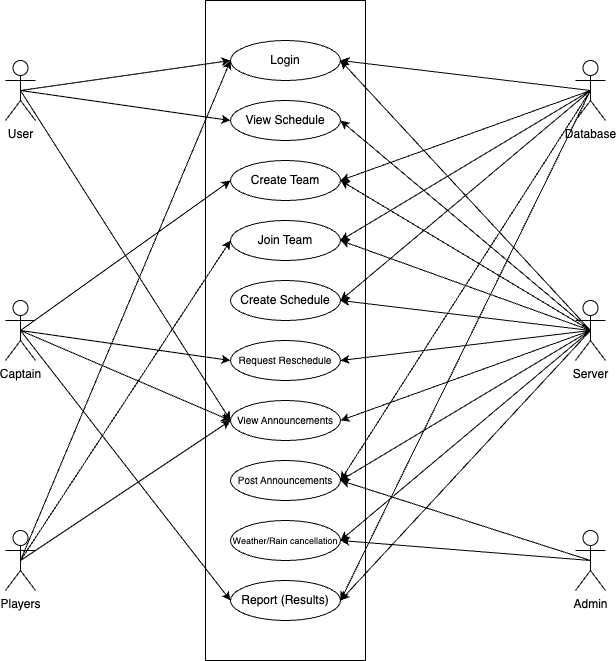
\includegraphics[width=\linewidth]{Use_case.png}
	\caption{Use Case List.}
	\label{fig:use_case}
\end{figure}
\pagebreak
\subsection{Individual Product Use Cases (PUC's)}
\begin{enumerate}
	\item Product Use Case Name: Login \\
	Trigger: User enters their username and password.\\
	Preconditions: Client is not logged in to the system with an existing account.\\
	Actors: User, Captain, Player, Database, Server.\\
	Outcome: If the username and password is a match with an account in
	the database, the user is logged in. If not, then the user is prompted
	to try again, reset password (if username exists) or create an account.
	\item Product Use Case Name: View Schedule \\
	Trigger: User interacts with the view schedule prompt.\\
	Preconditions: N/A (All users can view schedule)\\
	Actors: User, Database, Server
	Outcome: Page opens up with the schedule for the GSA softball league season.
	\item Product Use Case Name: View Standings \\
	Trigger: User interacts with View standings prompt.\\
	Preconditions: N/A (All users can view standings)\\
	Actors: User, Database, Server.\\
	Outcome: The standings for the GSA softball league season is displayed.
	\item Product Use Case Name: Create team \\
	Trigger: User request to make a team with team info.\\
	Preconditions: Client is logged in to the system as a Captain.\\
	Actors: User, Captain, Database, Server.\\
	Outcome: If the team name is unique and the user is not already an existing member
	of another team, the team is created with the user as the Captain of the team.
	\item Product Use Case Name: Join team \\
	Trigger: User request to join an already existing team\\
	Preconditions: User is logged into the system, the user is not part of an
	already existing team, and team being requested exists.\\
	Actors: User, Player, Database, Server.\\
	Outcome: If the user is logged in and is not a member of an already existing team, then
	the user will receive a request to fill out the waiver if the team exists. Upon completion,
	the user becomes a member of that team.
	\item Product Use Case Name: Create Schedule \\
	Trigger: Registration deadline is past due.\\
	Preconditions: Teams are registered in the league and meet the team conditions.\\
	Actors: Server.\\
	Outcome: The system uses the team preferences and creates a schedule with all open slots.
	\item Product Use Case Name: Request Reschedule \\
	Trigger: Captain interacts with the reschedule prompt at least 24 hours before the start time.\\
	Preconditions: Team exists and has a scheduled game.\\
	Actors: User, Captain, Database, Server.\\
	Outcome: If the user is a Captain and makes a request on an existing game at least 24 hours before
	the start, the Captain is able to view available slots for the game. Upon choosing an empty slot, the
	game schedule is updated.
	\item Product Use Case Name: View Announcements \\
	Trigger: User interacts with view announcement prompt.\\
	Preconditions: N/A (All users can view announcements).\\
	Actors: User, Captain, Player, Database, Server.\\
	Outcome: The announcements for the GSA softball league season is displayed.
	\item Product Use Case Name: Post announcements \\
	Trigger: User interacts with the post announcement prompt.\\
	Preconditions: User must me logged in as an Admin.\\
	Actors: User, Admin, Database, Server.\\
	Outcome: If the user is logged in as an admin, and enters all the necessary information to complete
	the required sections for the announcements, the announcements is created and published on the GSA
	softball league platform.
	\item Product Use Case Name: Rain cancellation/Override \\
	Trigger: User interacts with the Override prompt.\\
	Preconditions: User must me logged in as an Admin.\\
	Actors: User, Admin, Database, Server.\\
	Outcome: If the user is logged in as an admin, the user is able to cancel games or move then to open
	slots. Upon completion, the schedule is updated.
	\item Product Use Case Name: Report \\
	Trigger: User interacts with the report prompt.\\
	Preconditions: The user must be logged in as a Captain and the duration of a game must be elapsed after
	the scheduled start time.\\
	Actors: User, Captain, Database, Server.\\
	Outcome: If the user is logged in as a captain, and the duration of a game has been elapsed since the 
	start time, then the Captain is able to update the status of the game with results. Upon completion 
	the standings and game results are updated on the system.
\end{enumerate}


\section{Functional Requirements}
\subsection{Functional Requirements}
\textbf{Requirement \#:} 1 \quad \textbf{Requirement Type:} 9 \quad \textbf{Event/Use Case:} 1 \\
\textbf{Description:} The platform shall provide a login system where users enter credentials (username, password) to access the system.\\
\textbf{Rationale:} Ensures secure access to the platform and role-specific functionality.\\
\textbf{Fit Criterion:} No unauthorized users are able to log in and access role-based features after entering credentials.\\
\textbf{Customer Satisfaction:} 5 \quad\quad \textbf{Customer Dissatisfaction:} 5 \\
\noindent\rule{\textwidth}{1pt}

\textbf{Requirement \#:} 2 \quad \textbf{Requirement Type:} 9 \quad \textbf{Event/Use Case:} 1 \\
\textbf{Description:} The platform shall distinguish between different user roles (commissioner, captain, player) and role-specific access after login.\\
\textbf{Rationale:}  Provides tailored access to players, captains, admin.\\
\textbf{Fit Criterion:} Different user-roles only have access to the features assigned to their roles after login.\\
\textbf{Customer Satisfaction:} 5 \quad\quad \textbf{Customer Dissatisfaction:} 5 \\
\noindent\rule{\textwidth}{1pt}

\textbf{Requirement \#:} 3 \quad \textbf{Requirement Type:} 9 \quad \textbf{Event/Use Case:} 2 \\
\textbf{Description:} The platform shall allow users to view the game schedule including date, time, location, opponent.\\
\textbf{Rationale:} Facilitates easy access to schedule information to provide league members with aligned game information.\\
\textbf{Fit Criterion:} Schedules and game information are viewable by users.\\
\textbf{Customer Satisfaction:} 5 \quad\quad \textbf{Customer Dissatisfaction:} 5\\
\noindent\rule{\textwidth}{1pt}

\textbf{Requirement \#:} 4 \quad \textbf{Requirement Type:} 9 \quad \textbf{Event/Use Case:} 3 \\
\textbf{Description:} The platform shall provide an accurate display of league standings for all registered users.\\
\textbf{Rationale:} Keeps league members informed of team rankings.\\
\textbf{Fit Criterion:} League standings are updated accurately, automatically and visible to logged-in users.\\
\textbf{Customer Satisfaction:} 4 \quad\quad \textbf{Customer Dissatisfaction:} 4\\
\noindent\rule{\textwidth}{1pt}

\textbf{Requirement \#:} 5 \quad \textbf{Requirement Type:} 9 \quad \textbf{Event/Use Case:} 4 \\
\textbf{Description:} The platform shall allow captains to create a team by entering team details and submitting for registration.\\
\textbf{Rationale:} Enables team formation and league participation.\\
\textbf{Fit Criterion:} Captains can create a team, and details are stored in the system.\\
\textbf{Customer Satisfaction:} 5 \quad\quad \textbf{Customer Dissatisfaction:} 5\\
\noindent\rule{\textwidth}{1pt}

\textbf{Requirement \#:} 6 \quad \textbf{Requirement Type:} 9 \quad \textbf{Event/Use Case:} 5 \\
\textbf{Description:} The platform shall allow players to request to join a team, and notify the captain for approval.\\
\textbf{Rationale:} Simplifies team membership management and formation.\\
\textbf{Fit Criterion:} Players can submit join requests, and captains can approve or reject them and the system automatically updates the roster.\\
\textbf{Customer Satisfaction:} 4 \quad\quad \textbf{Customer Dissatisfaction:} 5\\
\noindent\rule{\textwidth}{1pt}

\textbf{Requirement \#:} 7 \quad \textbf{Requirement Type:} 9 \quad \textbf{Event/Use Case:} 6 \\
\textbf{Description:} The platform shall automatically generate the season game schedule based on team availability and preferences.\\
\textbf{Rationale:} Automates scheduling for league to begin with improved efficiency.\\
\textbf{Fit Criterion:} The system generates a schedule that gives all teams equal games and factors in team preferences.\\
\textbf{Customer Satisfaction:} 5 \quad\quad \textbf{Customer Dissatisfaction:} 5\\
\noindent\rule{\textwidth}{1pt}

\textbf{Requirement \#:} 8 \quad \textbf{Requirement Type:} 9 \quad \textbf{Event/Use Case:} 7 \\
\textbf{Description:} The platform shall allow captains to request a reschedule by selecting a new time slots for an existing game.\\
\textbf{Rationale:} Enables flexibility and error-handling in scheduling.\\
\textbf{Fit Criterion:} Captains can successfully submit reschedule requests, and the system tracks pending requests.\\
\textbf{Customer Satisfaction:} 4 \quad\quad \textbf{Customer Dissatisfaction:} 5\\
\noindent\rule{\textwidth}{1pt}

\textbf{Requirement \#:} 9 \quad \textbf{Requirement Type:} 9 \quad \textbf{Event/Use Case:} 8 \\
\textbf{Description:} The platform shall allow users to view league-wide announcements, lost and found, weather updates on the dashboard.\\
\textbf{Rationale:} Keeps users informed about important league updates. \\
\textbf{Fit Criterion:} Announcements are displayed in the users announncement dashboard.\\
\textbf{Customer Satisfaction:} 4 \quad\quad \textbf{Customer Dissatisfaction:} 3\\
\noindent\rule{\textwidth}{1pt}

\textbf{Requirement \#:} 10 \quad \textbf{Requirement Type:} 9 \quad \textbf{Event/Use Case:} 9 \\
\textbf{Description:} The platform shall allow administrators to post announcements that are visible to all users.\\
\textbf{Rationale:} Enables effective communication with all participants.\\
\textbf{Fit Criterion:} Administrators can post announcements to be viewable by players.\\
\textbf{Customer Satisfaction:} 3 \quad\quad \textbf{Customer Dissatisfaction:} 3\\
\noindent\rule{\textwidth}{1pt}

\textbf{Requirement \#:} 11 \quad \textbf{Requirement Type:} 9 \quad \textbf{Event/Use Case:} 10 \\
\textbf{Description:} The platform shall allow administrators to manually cancel or reschedule games due to weather conditions or accepted requests.\\
\textbf{Rationale:} Ensures timely communication for game rescheduling or cancellations.\\
\textbf{Fit Criterion:} Administrators can cancel or reschedule games, which updates the schedule, and teams are notified automatically. \\
\textbf{Customer Satisfaction:} 5 \quad\quad \textbf{Customer Dissatisfaction:} 4\\
\noindent\rule{\textwidth}{1pt}

\textbf{Requirement \#:} 12 \quad \textbf{Requirement Type:} 9 \quad \textbf{Event/Use Case:} 11 \\
\textbf{Description:} The platform shall allow captains to report game scores and forfeits by selecting a completed game and submitting the final result.\\
\textbf{Rationale:} Simplifies reporting and keeps standings up to date.\\
\textbf{Fit Criterion:} Captains can submit game results, and standings are updated automatically. \\
\textbf{Customer Satisfaction:} 4 \quad\quad \textbf{Customer Dissatisfaction:} 3\\

\section{Look and Feel Requirements}
\subsection{Appearance Requirements}
The platform must feature a modern, intuitive interface with consistent visual elements across all views to ensure ease of use.

\subsection{Style Requirements}
The platform shall follow a consistent color palette, typography, and layout to ensure ease of use, and improve accessibility by maintaining predictable design elements across the platform.

\section{Usability and Humanity Requirements}
\subsection{Ease of Use Requirements}
The product must be easy to use for graduate students.

\subsection{Personalization and Internationalization Requirements}
The platform must be tailored to Canadian English, using the metric system for measurements and adhering to local date and time formats.

\subsection{Learning Requirements}
The platform must provide clear instructions and tooltips on all views to help new users quickly learn how to navigate and use key features.\\

\noindent The platform must include easily accessible help documentation for users to learn how to perform tasks and resolve issues independently.


\subsection{Understandability and Politeness Requirements}
The platform must provide clear, straightforward navigation with simply labeled menus and buttons so that minimal prior knowledge is required.

\subsection{Accessibility Requirements}
The platform shall provide basic accessibility features, such as keyboard navigation and sufficient text contrast, to ensure usability for a wide range of users.

\section{Performance Requirements}
\subsection{Speed and Latency Requirements}
The platform must respond to user actions (e.g., scheduling, score reporting) within 1 second to contribute to user satisfaction and efficiency.

\subsection{Safety-Critical Requirements}
The platform must ensure the secure and accurate storage of player personal information and waivers, preventing data loss or corruption.

\subsection{Precision or Accuracy Requirements}
The platform must calculate and display the standings with 100\% accuracy.\\

\noindent The platform must accurately match game preferences with available slots to avoid conflicts or scheduling errors and maximize adhesion with team schedule preferences.

\subsection{Robustness or Fault-Tolerance Requirements}
The platform shall handle common errors (e.g., failed database connections) without crashing, and users shall be able to retry actions if errors occur.

\subsection{Capacity Requirements}
The platform must be able to store and handle the scheduling for at minimum 50 teams in the league to ensure scheduling handling and league expansion.

\subsection{Scalability or Extensibility Requirements}
The platform shall support up handling 50 teams without performance issues to ensure scheduling handling and website performance for a full league.

\subsection{Longevity Requirements}
The platform must use modern, widely supported web technologies to ensure long-term compatibility with future devices and browsers.

\section{Operational and Environmental Requirements}
\subsection{Expected Physical Environment}
The platform must be accessible on various devices, such as desktops, laptops, smartphones, and tablets.
The platform will also require a stable internet connection.
Servers are needed to store information in the database, such as team rosters, photos, etc.

\subsection{Wider Environment Requirements}
Although the platform will be accessible across various devices, we want our platform to be accessed across multiple browsers, such as Chrome, Safari, Firefox, Edge, etc.
Even if our platform is accessible by smartphones and tablets, it must have a responsive design that allows the user to reach all features when using a mobile device.

\subsection{Requirements for Interfacing with Adjacent Systems}
Our platform may need to integrate with payment gateways to handle payment management, such as PayPal.
It would be useful if our platform could integrate with popular calendar systems, such as Google Calendar.
There might be some features that could benefit from CSV / Excel import or export, such as roster data and match results.

\subsection{Productization Requirements}
Our platform must handle scaling well, such as an increased number of divisions, teams, players, etc.
Depending on the league, the managers should be able to manage anything related to game rules, so that the information is clear to users of the product (in this case, the players of the league).

\subsection{Release Requirements}
Version control is extremely important, previous platforms must be saved in version control so we can track changes and rollback if unnecessary.
Before any production release, thorough testing must be done to gather feedback. If possible, testing with real users would be the most beneficial.

\section{Maintainability and Support Requirements}
\subsection{Maintenance Requirements}
The platform should be updated regularly for fixing bugs, adding new features, and security patches.

\subsection{Supportability Requirements}
Any user who requires support should be directed to an email that handles issues with the platform.

\subsection{Adaptability Requirements}
An admin user should be able to change game rules within 2 minutes, such as swapping a team’s game schedule with another if needed.

\section{Security Requirements}
\subsection{Access Requirements}
There must be role-based access control. Administrator roles must have access to everything. Team managers should have access to team management. Players should be restricted to a degree.

\subsection{Integrity Requirements}
All data entered such as team rosters, game schedules, and scores must be validated for accuracy and completeness.

\subsection{Privacy Requirements}
Personal user data such as emails, phone numbers, etc., should be protected by encryption.

\subsection{Audit Requirements}
Logs of team history, game scores, roster updates, and game scheduling, should all be kept in case we ever need them to solve disputes.

\subsection{Immunity Requirements}
The platform should be protected against malicious web attacks.

\section{Cultural Requirements}
\subsection{Cultural Requirements}
The platform should support multiple languages so that the diverse league participants can switch to their preferred language. The platform should only display the local time of Hamilton, as it is assumed that all league participants are in the same region where the games are being hosted.

\section{Compliance Requirements}
\subsection{Legal Requirements}
Users who no longer want to be part of the league should be able to delete their data. The platform must accommodate for this within 2 minutes.

\subsection{Standards Compliance Requirements}
The platform must meet typical web standards, such as readable font, colours that are easy to look at, easy to navigate, etc.

\section{Open Issues}
\begin{itemize}
    \item \textbf{User Interface Design}: Some aspects of the user interface are yet to be fully defined. Specific visual elements and interaction flows will be determined in collaboration with stakeholders during the design phase.
    \item \textbf{User Interface Testing}: Details on the testing methodology for the user interface are still under discussion. The testing plan will include usability testing with users from the target audience to ensure ease of use.
    \item \textbf{User Payment Tracking Feature}: The implementation specifics for the payment tracking feature for staff are still being finalized. Considerations are being made regarding how the status of each player's payment will be updated and stored.
    \item \textbf{Integration of Existing Features}: There are open questions regarding the best approach to integrate and improve existing features from the current website in the new platform.
\end{itemize}

\section{Off-the-Shelf Solutions}
\subsection{Ready-Made Products}
There are no ready-made products that will be a part of our solution. The objective is to update and completely redesign the current softball league web-based platform. While features from the original platform will be transferred over to maintain continuity, the entire solution will be developed in-house based on updated requirements and best practices.

\subsection{Reusable Components}
While no third-party reusable components will be integrated, several features from the original platform, such as user authentication, team management, and scheduling, will be carried over to ensure continuity. These components will be updated and enhanced as part of the complete redesign to meet the new requirements.

\subsection{Products That Can Be Copied}
There are no external products that will be directly copied for this project. However, the redesign will reference the design and functional elements of the current website to maintain familiarity for existing users. Additionally, best practices from similar platforms will be researched and adapted to improve the user experience.


\section{New Problems}
\subsection{Effects on the Current Environment}
Implementing the new system will require a complete overhaul of the existing McMaster GSA softball league platform, which may cause temporary disruption to ongoing league activities. The outdated system will be replaced, and users accustomed to the old methods may face a learning curve during the transition. Additionally, migrating any existing data (such as player information, schedules, and standings) to the new platform will need to be handled carefully to avoid loss or corruption. However, the improved system will provide long-term benefits by reducing maintenance and manual input required by the commissioners and administrators. 
\subsection{Effects on the Installed Systems}
Since the current system is outdated integrating the new platform may require adjustments to the existing server infrastructure or cloud services. The new system will be built on modern technologies which may require updating the server environment to ensure compatibility with these technologies. If hosted on legacy systems, a migration to a cloud or updated hosting service might be required.
\subsection{Potential User Problems}
Users (commissioners, captains, players) who are familiar with the current platform may struggle with adapting to the new interface and features. Particularly, older users or users with less technical proficiency may have difficulty navigating the system or understanding new functionalities like the rescheduling workflow, leaderboard tracking, or player management. Proper documentation and user training will be necessary to ensure a smooth transition and reduce user frustration. Moreover, captains and commissioners may need additional guidance on using automated features like team creation, player approvals, and schedule rescheduling.
\subsection{Limitations in the Anticipated Implementation Environment That May
Inhibit the New Product}
The project must be compatible with various devices (desktop, tablet, mobile), which presents challenges in ensuring consistent performance and user experience across different screen sizes and browsers. Another potential limitation is the anticipated usage spikes, such as the heavy volume of rescheduling requests at the beginning of the season, which could strain the system. The hosting environment needs to handle potential scalability issues, and the system should be optimized for responsiveness during high-demand periods. There may also be limitations in integrating certain external services, such as payment verification systems, if APIs or infrastructure constraints arise.
\subsection{Follow-Up Problems}
After the initial launch of the new platform, follow-up issues may include bug fixes, additional feature requests, and ongoing user feedback that necessitates adjustments. Since the system will rely on certain automated processes (e.g., scheduling, score reporting), there may be edge cases or scenarios not accounted for during development, which would require post-launch refinements. Maintenance and updates to the platform will need to be addressed continuously to ensure smooth functionality, especially in response to league changes or growing participation numbers. Moreover, as the system expands, additional support or enhancements might be required to maintain security and efficiency.

\section{Tasks}

\subsection{Project Planning}
The platform’s development will follow a structured plan prioritizing the requirements as outlined in the SRS. The functional requirements have been grouped based on priority, with each group indicating the relevant requirement numbers. Non-functional requirements, such as look and feel, usability, and accessibility, will be applied throughout the project to ensure consistency across all phases.

\textbf{High Priority} – These features are critical for the functioning of the platform:
\begin{itemize}
    \item \textbf{User Authentication and Account Management} (Requirements \#1, \#2): Secure login and user roles (commissioner, captain, player).
    \item \textbf{Team Management} (Requirements \#5, \#6): Captains create teams, select divisions, and manage rosters. Players can request to join teams.
    \item \textbf{Schedule Generation} (Requirement \#7): Automatically generate schedules, ensuring even distribution and honoring team preferences for dates/times.
    \item \textbf{Score Reporting} (Requirements \#11, \#12): Captains report game scores and forfeits, updating standings automatically.
    \item \textbf{Rescheduling System} (Requirements \#8, \#11): Allow captains to reschedule games, with requests approved by commissioners. Handle conflict checks and queues for multiple requests.
\end{itemize}

\textbf{Medium Priority} – These features enhance the user experience but are not critical to the platform’s core functionality:
\begin{itemize}
    \item \textbf{Player Login and Team Requests} (Requirement \#6): Players can log in, view team information, and request to join teams.
    \item \textbf{Rescheduling Queue Management} (Requirement \#8): Manage multiple rescheduling requests and enforce time restrictions (e.g., within 24 hours of a game).
    \item \textbf{Announcements} (Requirements \#9, \#10): Commissioners post league-wide announcements for all users.
\end{itemize}

\textbf{Low Priority} – Features that are “nice to have” but not necessary for platform operation:
\begin{itemize}
    \item \textbf{UI/UX Enhancements} (Non-functional requirement): A modern interface, cleaner design, weekly schedule tabs, and alternating colors for easier reading.
    \item \textbf{Lost and Found Feature} (Non-functional requirement): Allow users to report and check lost items.
    \item \textbf{Waiver System} (Non-functional requirement): Integrate waivers with payment status tracking.
\end{itemize}

\subsection{Planning of the Development Phases}
Development will be divided into phases, with each phase focused on implementing the functional requirements in order of priority. Each phase includes start and end dates based on your project schedule:

\subsubsection{Phase 1: Requirement Gathering and Initial Planning}
\textit{Start: September 10, 2024 | End: October 9, 2024}
\begin{itemize}
    \item Meet with stakeholders to determine the functional and non-functional requirements of the platform.
    \item Prioritize requirements based on their criticality to the project.
    \item Document the initial project plan, setting up deadlines for each phase.
\end{itemize}

\subsubsection{Phase 2: Proof of Concept and Design}
\textit{Start: October 10, 2024 | End: November 22, 2024}
\begin{itemize}
    \item Develop and demonstrate a proof of concept for high-priority features, including user authentication, team management, and scheduling (Requirements \#1, \#2, \#5, \#7).
    \item Finalize the design document and refine it based on stakeholder feedback.
\end{itemize}

\subsubsection{Phase 3: Core Development}
\textit{Start: November 23, 2024 | End: January 15, 2025}
\begin{itemize}
    \item Implement high-priority features, including team management, scheduling, and score reporting (Requirements \#5, \#7, \#11, \#12).
    \item Begin the integration of features from the existing platform where applicable.
\end{itemize}

\subsubsection{Phase 4: Verification, Validation, and Revision}
\textit{Start: January 16, 2025 | End: March 7, 2025}
\begin{itemize}
    \item Test the platform against the documented requirements.
    \item Present the initial version (Revision 0) and gather feedback for improvement.
\end{itemize}

\subsubsection{Phase 5: Final Development and Demonstration}
\textit{Start: March 8, 2025 | End: March 30, 2025}
\begin{itemize}
    \item Finalize medium- and low-priority features, such as announcements and UI/UX improvements (Requirements \#9, \#10, non-functional requirements).
    \item Prepare for the final demonstration and present the platform.
\end{itemize}

\subsubsection{Phase 6: Documentation and Wrap-Up}
\textit{Start: April 1, 2025 | End: April 2, 2025}
\begin{itemize}
    \item Complete all project documentation.
    \item Submit the final deliverables, including the user guide and source code.
\end{itemize}


\section{Migration to the New Product}
\subsection{Requirements for Migration to the New Product}
To migrate from the existing platform to our redesign involves several key steps to ensure that the transfer of all relevant data, features, and functionalities is seamless and complete:

\begin{itemize}
    \item \textbf{Data Preservation}: All current data from the existing platform must be preserved and migrated to the new platform. The specific data to be transferred will be confirmed through consultation with the current platform administrator, ensuring that only the necessary and relevant data is included in the migration.
    \item \textbf{Feature Continuity}: Ensure that all features present in the original platform are retained in the redesigned version, with enhancements and improvements where applicable.
    \item \textbf{Minimizing Downtime}: The softball season begins in April, which falls around when the project is expected to be completed. Due to this tight deadline, the migration process should be planned to minimize downtime for users, ensuring that the transition is as smooth as possible with minimal impact on league operations.
\end{itemize}

\subsection{Data That Has to be Modified or Translated for the New System}
During the migration process, specific data elements may need to be modified or translated to align with the new platform's structure and data requirements:

\begin{itemize}
    \item \textbf{User Accounts and Roles}: The login system needs a complete redesign. User account information, including usernames, passwords, and roles (commissioner, captain, player), will need to be reformatted to match the requirements of the new authentication system.
    \item \textbf{Team and Match Data}: Team rosters, match schedules, and historical results may require adjustments to fit the new database schema. This may involve reformatting data fields or translating old data structures to new formats.
\end{itemize}

\section{Costs}
The capstone supervisor expressed minimizing costs. Our approach will be done with free frameworks, such as React.js, and affordable hosting plans such as AWS or Google Cloud. Our team will emphasize core functionality, and avoid creating unnecessary features and costs that could undermine the product goal. By following these cost-conscious strategies, the project can stay within budget while delivering a functional and scalable platform.

\section{User Documentation and Training}
\subsection{User Documentation Requirements}
\begin{itemize}
    \item \textbf{Comprehensive User Guide}: Create a detailed user manual page tab that outlines:
    \begin{itemize}
        \item \textbf{Getting Started}: Instructions on how to register, create teams, and navigate the platform before delving deep into more advanced features.
        \item \textbf{Feature Descriptions}: Written and visual explanations of each feature, such as team management, scheduling, score tracking, etc.
        \item \textbf{FAQs}: Address common questions and troubleshooting tips to help users resolve issues independently. If unresolved, prompt users to email for more support or direct them to the discussions page.
    \end{itemize}
    \item \textbf{Interactive Tutorials}: Create pop-up icons that demonstrate key functionalities, making it easier for both new and existing users to understand how to use the platform effectively.
\end{itemize}

\subsection{Training Requirements}
\begin{itemize}
    \item \textbf{Help Support Desk}: A dedicated support email or live chat feature where users can ask questions or report issues with someone real.
    \item \textbf{Feedback Section}: Implement a section where users can provide feedback through open-ended surveys to help improve the platform.
    \item \textbf{Discussion}: A section where users can publicly post their questions and other users are free to answer them.
\end{itemize}

\section{Waiting Room}
For the softball league platform, the “waiting room” will most likely be the feature for players who have registered, but do not have a pre-formed team. These players are called “free agents,” who may be added to teams later once all team rosters are confirmed. This concept is similar to how IMLeague is handled, which is the McMaster Intramural League platform. For example, a student desires to play softball and registers for the platform. As pre-formed teams are registered and confirmed, this student will be assigned to one of the teams that have extra space on their roster. Hence, they are “waiting” for a team to join.

\section{Ideas for Solution}
Players who sign up without a pre-formed team will be placed in a waiting room, designating them as “free agents.” This waiting room is a holding area until all team rosters are confirmed. Other teams can choose from this holding area if they need any players before the final roster confirmation date. However, all players will eventually be auto-assigned to a team if the waiting room is still non-empty. Players from the waiting room will be notified of status updates. Players who register late will also be automatically assigned from the waiting room.

Therefore, we need a database to hold the status of each player in the waiting room. On the front user interface, the waiting room should be displayed to all users, so teams can see available free agents. For users with team manager permissions, they will be able to invite free agents from the waiting room to their teams if desired.


\newpage{}
\section*{Appendix --- Reflection}

The information in this section will be used to evaluate the team members on the
graduate attribute of Lifelong Learning.  Please answer the following questions:

\begin{enumerate}
  \item What knowledge and skills will the team collectively need to acquire to
  successfully complete this capstone project?  Examples of possible knowledge
  to acquire include domain specific knowledge from the domain of your
  application, or software engineering knowledge, mechatronics knowledge or
  computer science knowledge.  Skills may be related to technology, or writing,
  or presentation, or team management, etc.  You should look to identify at
  least one item for each team member.
  \item For each of the knowledge areas and skills identified in the previous
  question, what are at least two approaches to acquiring the knowledge or
  mastering the skill?  Of the identified approaches, which will each team
  member pursue, and why did they make this choice?
\end{enumerate}

\end{document}